% XCircuit output "tx_angle.tex" for LaTeX input from tx_angle.ps
\def\putbox#1#2#3#4{\makebox[0in][l]{\makebox[#1][l]{}\raisebox{\baselineskip}[0in][0in]{\raisebox{#2}[0in][0in]{\scalebox{#3}{#4}}}}}
\def\rightbox#1{\makebox[0in][r]{#1}}
\def\centbox#1{\makebox[0in]{#1}}
\def\topbox#1{\raisebox{-0.60\baselineskip}[0in][0in]{#1}}
\def\midbox#1{\raisebox{-0.20\baselineskip}[0in][0in]{#1}}
   \scalebox{1}{
   \normalsize
   \parbox{6.20833in}{
   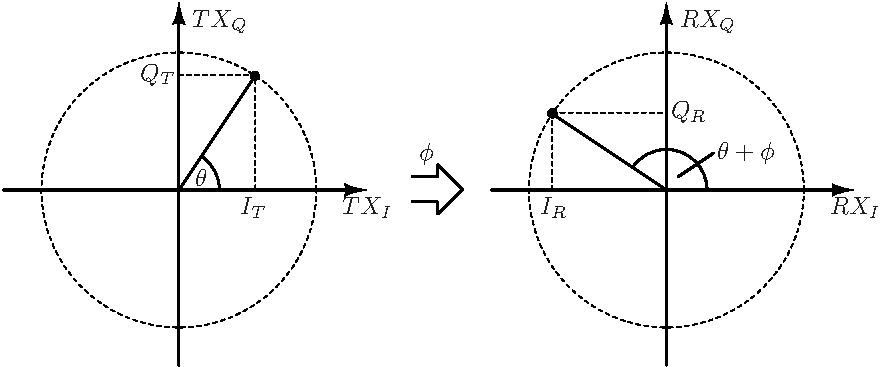
\includegraphics[scale=1]{tx_angle}\\
   % translate x=416 y=416 scale 0.38
   \putbox{2.31in}{1.06in}{1.20}{$TX_I$}%
   \putbox{1.31in}{2.31in}{1.20}{$TX_Q$}%
   \putbox{1.37in}{1.25in}{1.20}{\centbox{$\theta$}}%
   \putbox{5.56in}{1.06in}{1.20}{$RX_I$}%
   \putbox{4.56in}{2.31in}{1.20}{$RX_Q$}%
   \putbox{4.81in}{1.47in}{1.20}{\midbox{$\theta+\phi$}}%
   \putbox{2.87in}{1.42in}{1.20}{\centbox{$\phi$}}%
   \putbox{1.72in}{1.06in}{1.20}{\centbox{$I_T$}}%
   \putbox{1.20in}{1.99in}{1.20}{\rightbox{\midbox{$Q_T$}}}%
   \putbox{3.72in}{1.06in}{1.20}{\centbox{$I_R$}}%
   \putbox{4.50in}{1.74in}{1.20}{\midbox{$Q_R$}}%
   } % close 'parbox'
   } % close 'scalebox'
   \vspace{-\baselineskip} % this is not necessary, but looks better
